\chapter{Results}

The following section is supposed to provide a scientific scenario and three corresponding sample sessions in which the earthEngineGrabR can be used to acquire remote sensing data to meet a specific question. The emphasis of this section lies on how to use the earthEngineGrabR and gives tips and tricks on how to apply the package.

\section{Szenario}

Imagine, you are a scientist involved with the MIKE Programm (Monitoring the Illegal Killing of Elephants). 


\begin{wrapfigure}{r}{0.5\textwidth}
	\begin{center}
		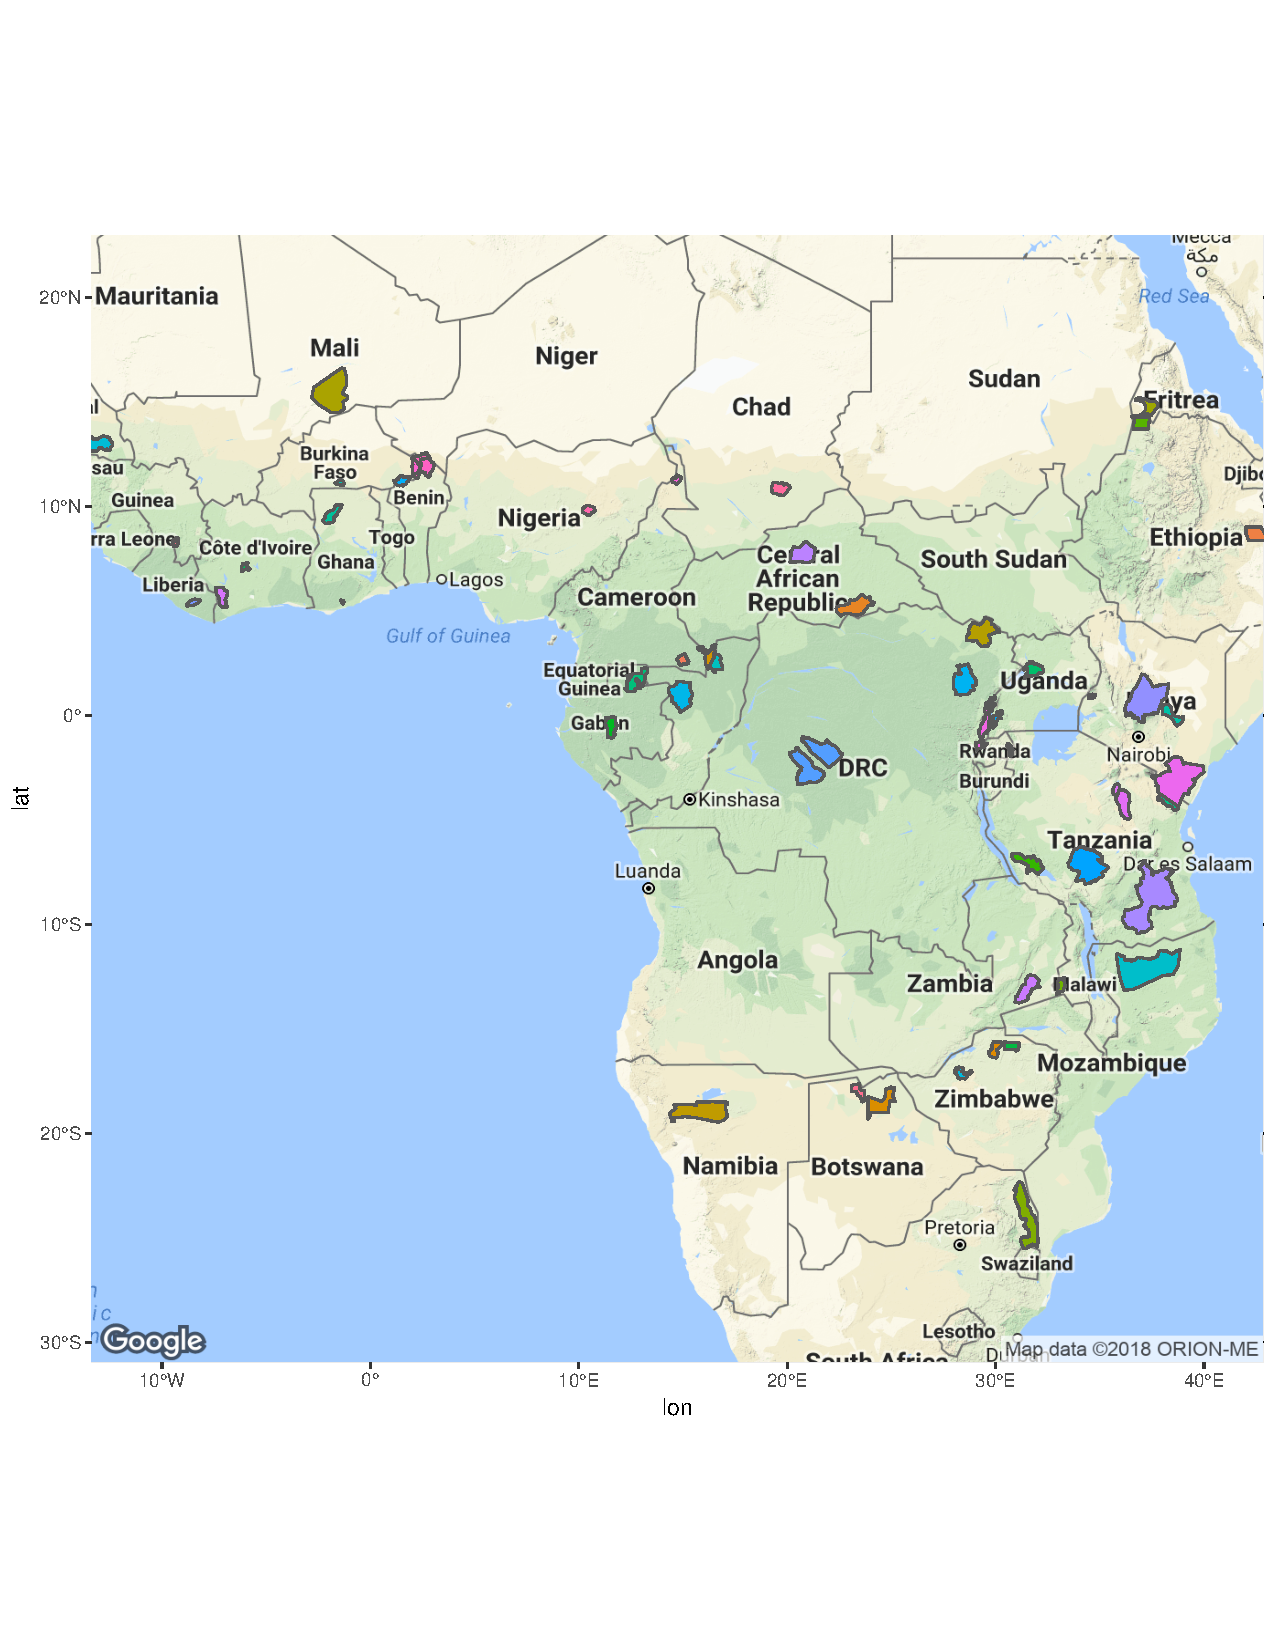
\includegraphics[width=7cm]{images/territories.pdf}
	\end{center}
	\caption{Elephant territories for the Great Elephant Census aerial survey}
	\label{territories}
\end{wrapfigure}
% \vskip 2em%

Your object of investigation is to find covariates for the intensity of illegally killed elephants in Africa. You have access to data collected within the Great Elephant Census, a continent-wide aerial survey counting the number and distribution of elephants within there territories. Figure \ref{territories} shows the study area. Each region corresponds to a territory, and for each territory, you have the aggregated number of illegally killed elephants. To run your statistical model in R and find influential covariates you need further environmental variables derived from satellite imagery like the topography, land-use, and precipitation. 


Because the study area is fragmented and of large-scale at the same time it would require significant effort to use one of the search and order tools like the Earth Explorer, to acquire and prepare the remote sensing data for your analysis. You would have to download a multitude of tiles for each of your environmental variables to cover the study area. Next, you would have to integrate, merge and aggregate all this data in an external GIS application before you start your actual analysis in R. But fortunately, you know, that one of your colleagues lately used a new R packages, some "graber" that greatly simplified his data acquisition process and you are desperate enough to give it a try. After some googling, you find the earthEngineGrabR and the corresponding Git Hup page, which describes how to apply for an EE account and how to install the required dependencies for the package. Because you have GDAL and Python already installed, you only install the sf R package and wait a few hours for the acknowledgement e-mail from Google, that you or your Google Account is now a trusted tester of the EE. Now you are ready to use the earthEngineGrabR.

\section{Large-scale analysis}

First, install the package from Git Hup with the \texttt{install\_githup()} function form the devtools package.

\begin{lstlisting}
library(devtools)
install_github("JesJehle/earthEngineGrabR")
\end{lstlisting}

After installing the package the first step is to initialize the package with \texttt{ee\_grab\_init()}. 

\begin{lstlisting}
library(earthEngineGrabR)
ee_grab_init()
\end{lstlisting}

As described in the method section the \texttt{ee\_grab\_init()} function installs all additionally required dependencies and guides the user through the authentication processes to activate the different API's. To authenticate to the API the user has to log in to his Google account and allow the API to access data on googles servers on the user's behalf. 


If the Google account is verified and the permission is granted, the user is directed to an authentification token. This token is manually copied and pasted into a running command line script, which creates persistent credentials. Later, the credentials are used to authenticate a request to the API. To simplify this procedure, the \texttt{ee\_grab\_init()} function successively opens a browser window to log into the Google account and a corresponding command line window to enter the token (see figure \ref{install}). 

This process is repeated for each API. If the function runs successfully, all needed credentials are stored for further sessions. Because some of the credentials expire after a few hours, a reauthentication is necessary. This process is handled automatically inside the \texttt{ee\_grab()} function. If a reauthentication is needed the function opens a browser window and the user is asked to log in to his Google account. The creation of credentials is automated, and there is no need to copy or paste the token manually.

\begin{center}
	\begin{figure}[h]
		\begin{center}
			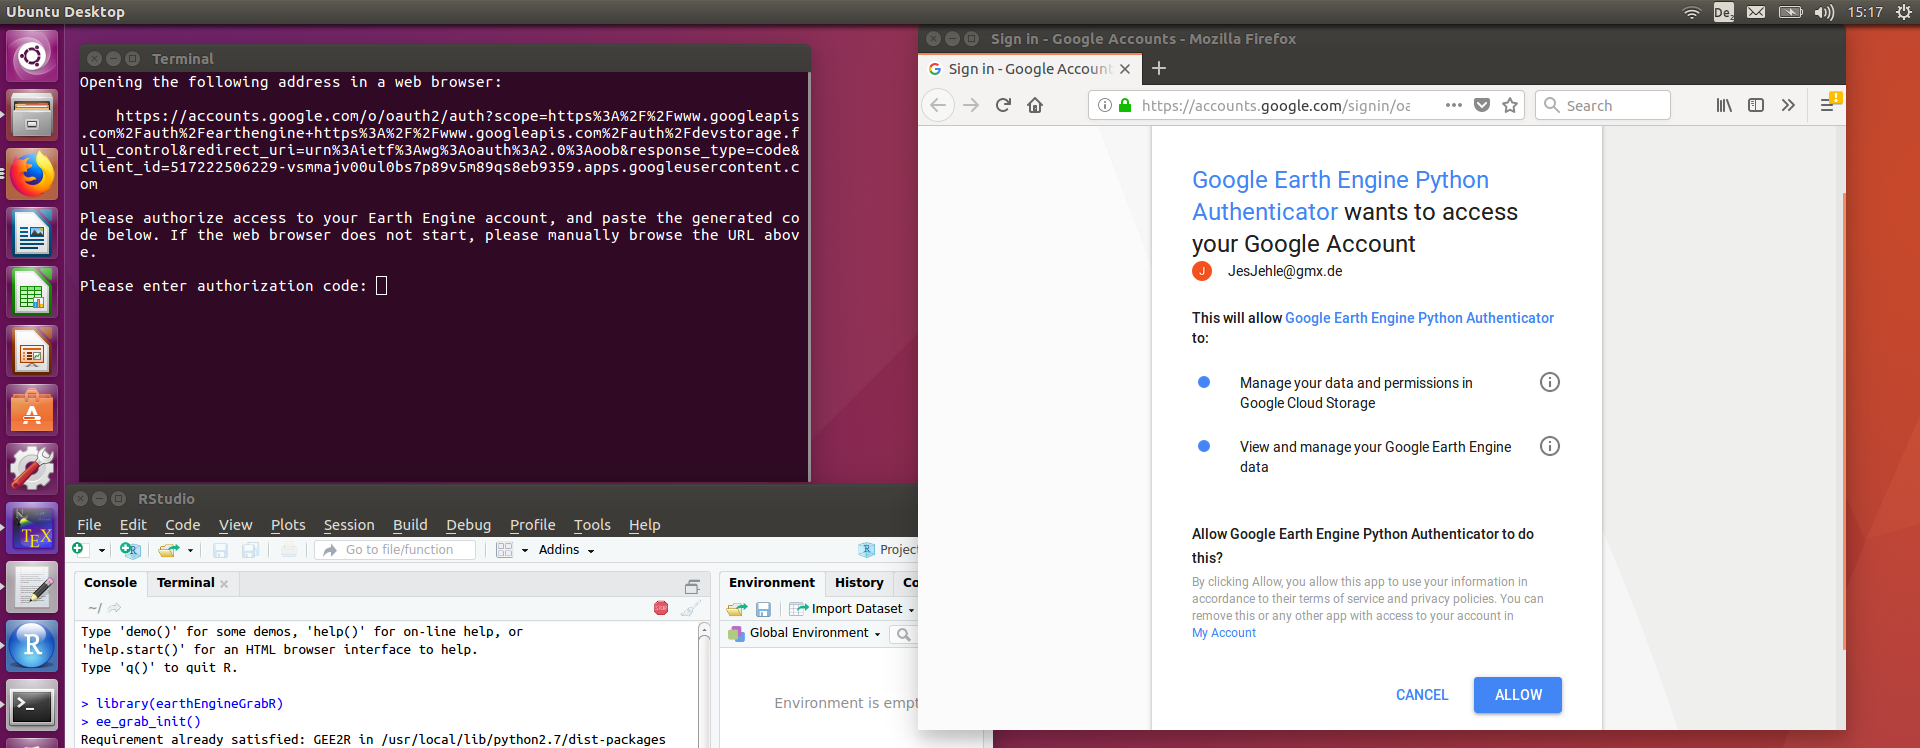
\includegraphics[width=15cm]{images/install_authentication.png}
			\caption{Example of the authentication process for the EE API}
			\label{install}
		\end{center}
	\end{figure}
	% \vskip 2em%
\end{center}



To acquire the data next the \texttt{ee\_grab()} function is used. The target is the path to the shapefile of the elephant territories shown in figure \ref{territories}. The products argument takes a list of earth engine data product-functions. Each function specifies one particular data product, and it's necessary parameter. The name of the function is \texttt{eeProduct\_ }followed by the source of the data products, underscore the name of the data product. For example: \texttt{eeProduct\_modis\_treecover()}. Because all data products start with \texttt{eeProduct\_ }, by simply typing \texttt{eeProduct\_ }, R's autocomplete function opens a drop-down menu of all available data products. Furthermore, the selection of a product in the menu displays a little description of the product and list their possible parameters. For more Information on a particular data product simply open the documentation of the function by pressing F1, or use equivalent methods. This way, it's possible to browse through the products, without any additional metadata outside of R. Additionally the functions provide default parameter values, which allow a test run without the need of specifying any parameter. While this procedure provides a user-friendly selection of available data products with their corresponding parameters, it also minimises potential typing and spelling errors.

After browsing through the data products, you choose the modis-tree-cover product for the year 2000 to 2005. You are further interested in the mean tree cover between this period and also want the mean tree cover in each of the elephant territories. Because the default value for the time reducer and the spatial reducer is mean you only need to specify the time interval parameter with a vector of the start and end-year (\texttt{timeInterval = c(2000, 2005)}). You are further interested in a potential correlation of the accessibility to populated areas and the illegally killed elephant. Therefore you additionally choose the oxford-accessibility product. The information displayed by the R's auto compete feature reveals only one possible parameter - spatialReducer - and by requesting the documentation of the function, you learn that this data product is only available for the year 2015, and therefore has no temporal resolution to aggregate. Again, you choose the mean accessibility in each territory by using the default value of the parameter and add the product function to the list. The last argument specifies the resolution in meters as edge length. 


\begin{lstlisting}

africa_elephant_data <- ee_grab(
target = system.file("data/territories.shp", package="earthEngineGrabR"),
products = list(
eeProduct_modis_treeCover(yearIntervall = c(2000, 2005)),
eeProduct_oxford_accessibility()
),
resolution = 1000
)
\end{lstlisting}


The resolution parameter sets the resolution of the processed data in EE and applies for all products. A value smaller than the native resolution of the data product results in EE resampling the data with the default nearest neighbour method, values higher result in a pixel aggregation with a default method mean. In the documentation, you learned that the native resolution of the tree cover product is 250 m while the accessibility products provide a resolution of 30 m. Because the area of the elephant territories is of large-scale (mean area of the regions is 9862 km$^2$), you choose 1000 m as the scale of your analysis. The resolution parameter actively controls the scope of computation and out of this the processing time. Therefore it's a good choice to not unnecessarily set him too low. 
Since all parameters are set, the function can be executed. 
During the processing the function prints info corresponding to the state of the upload, the processing and the download of each data product. With the verbose = FALSE, this behaviour can be avoided. 

As most processes of the function call are performed on Googles servers, the execution time depends strongly on the throughput of your analysis on the servers and only slightly on the performance of your local machine. However, because of the upload and download process during the function execution, deficient internet speed (1 Mbit/s in download and 0.1 Mbit/s in upload) can work as a bottleneck, particularly during the upload process. 
On a 64-bit ubuntu machine with 8 Gbit of RAM, 4 cores with 2.40 GHz and internet speed of 10 Mbit/s in download and 1Mbit/s in upload the \texttt{ee\_grab()} function took 55 s to execute. All further time measurements refer to this setting.
The output of the \texttt{ee\_grab()} function is an object of class sf.  The output always contains all properties of the original target vector data with the added data products and an additional geometry column as shown in table \ref{output}.

\begin{table}[h]
	\begin{tabularx}{\textwidth}{|l|l|l|c|c|c|}
		\hline
		id & sitecode & name & tree Cover & accessibility & geometry \\
		\hline
		1  & AKG  & Akagera & 15 & 138.4 & MULTIP. (30.5 -1.\\
		2 & DZA  & Dzanga-Sangha & 76.4 & 858.9 & MULTIP. (16.06 2.\\
		3 & MCH  & Murchison Falls & 25.0 & 146.1 & MULTIP. (32.1 2.\\
		
		\hline
	\end{tabularx}
	\caption{Example output of the \texttt{ee\_grab()} function}
	\label{output}
\end{table}


\begin{center}
	\begin{figure}[H]
		\begin{center}
			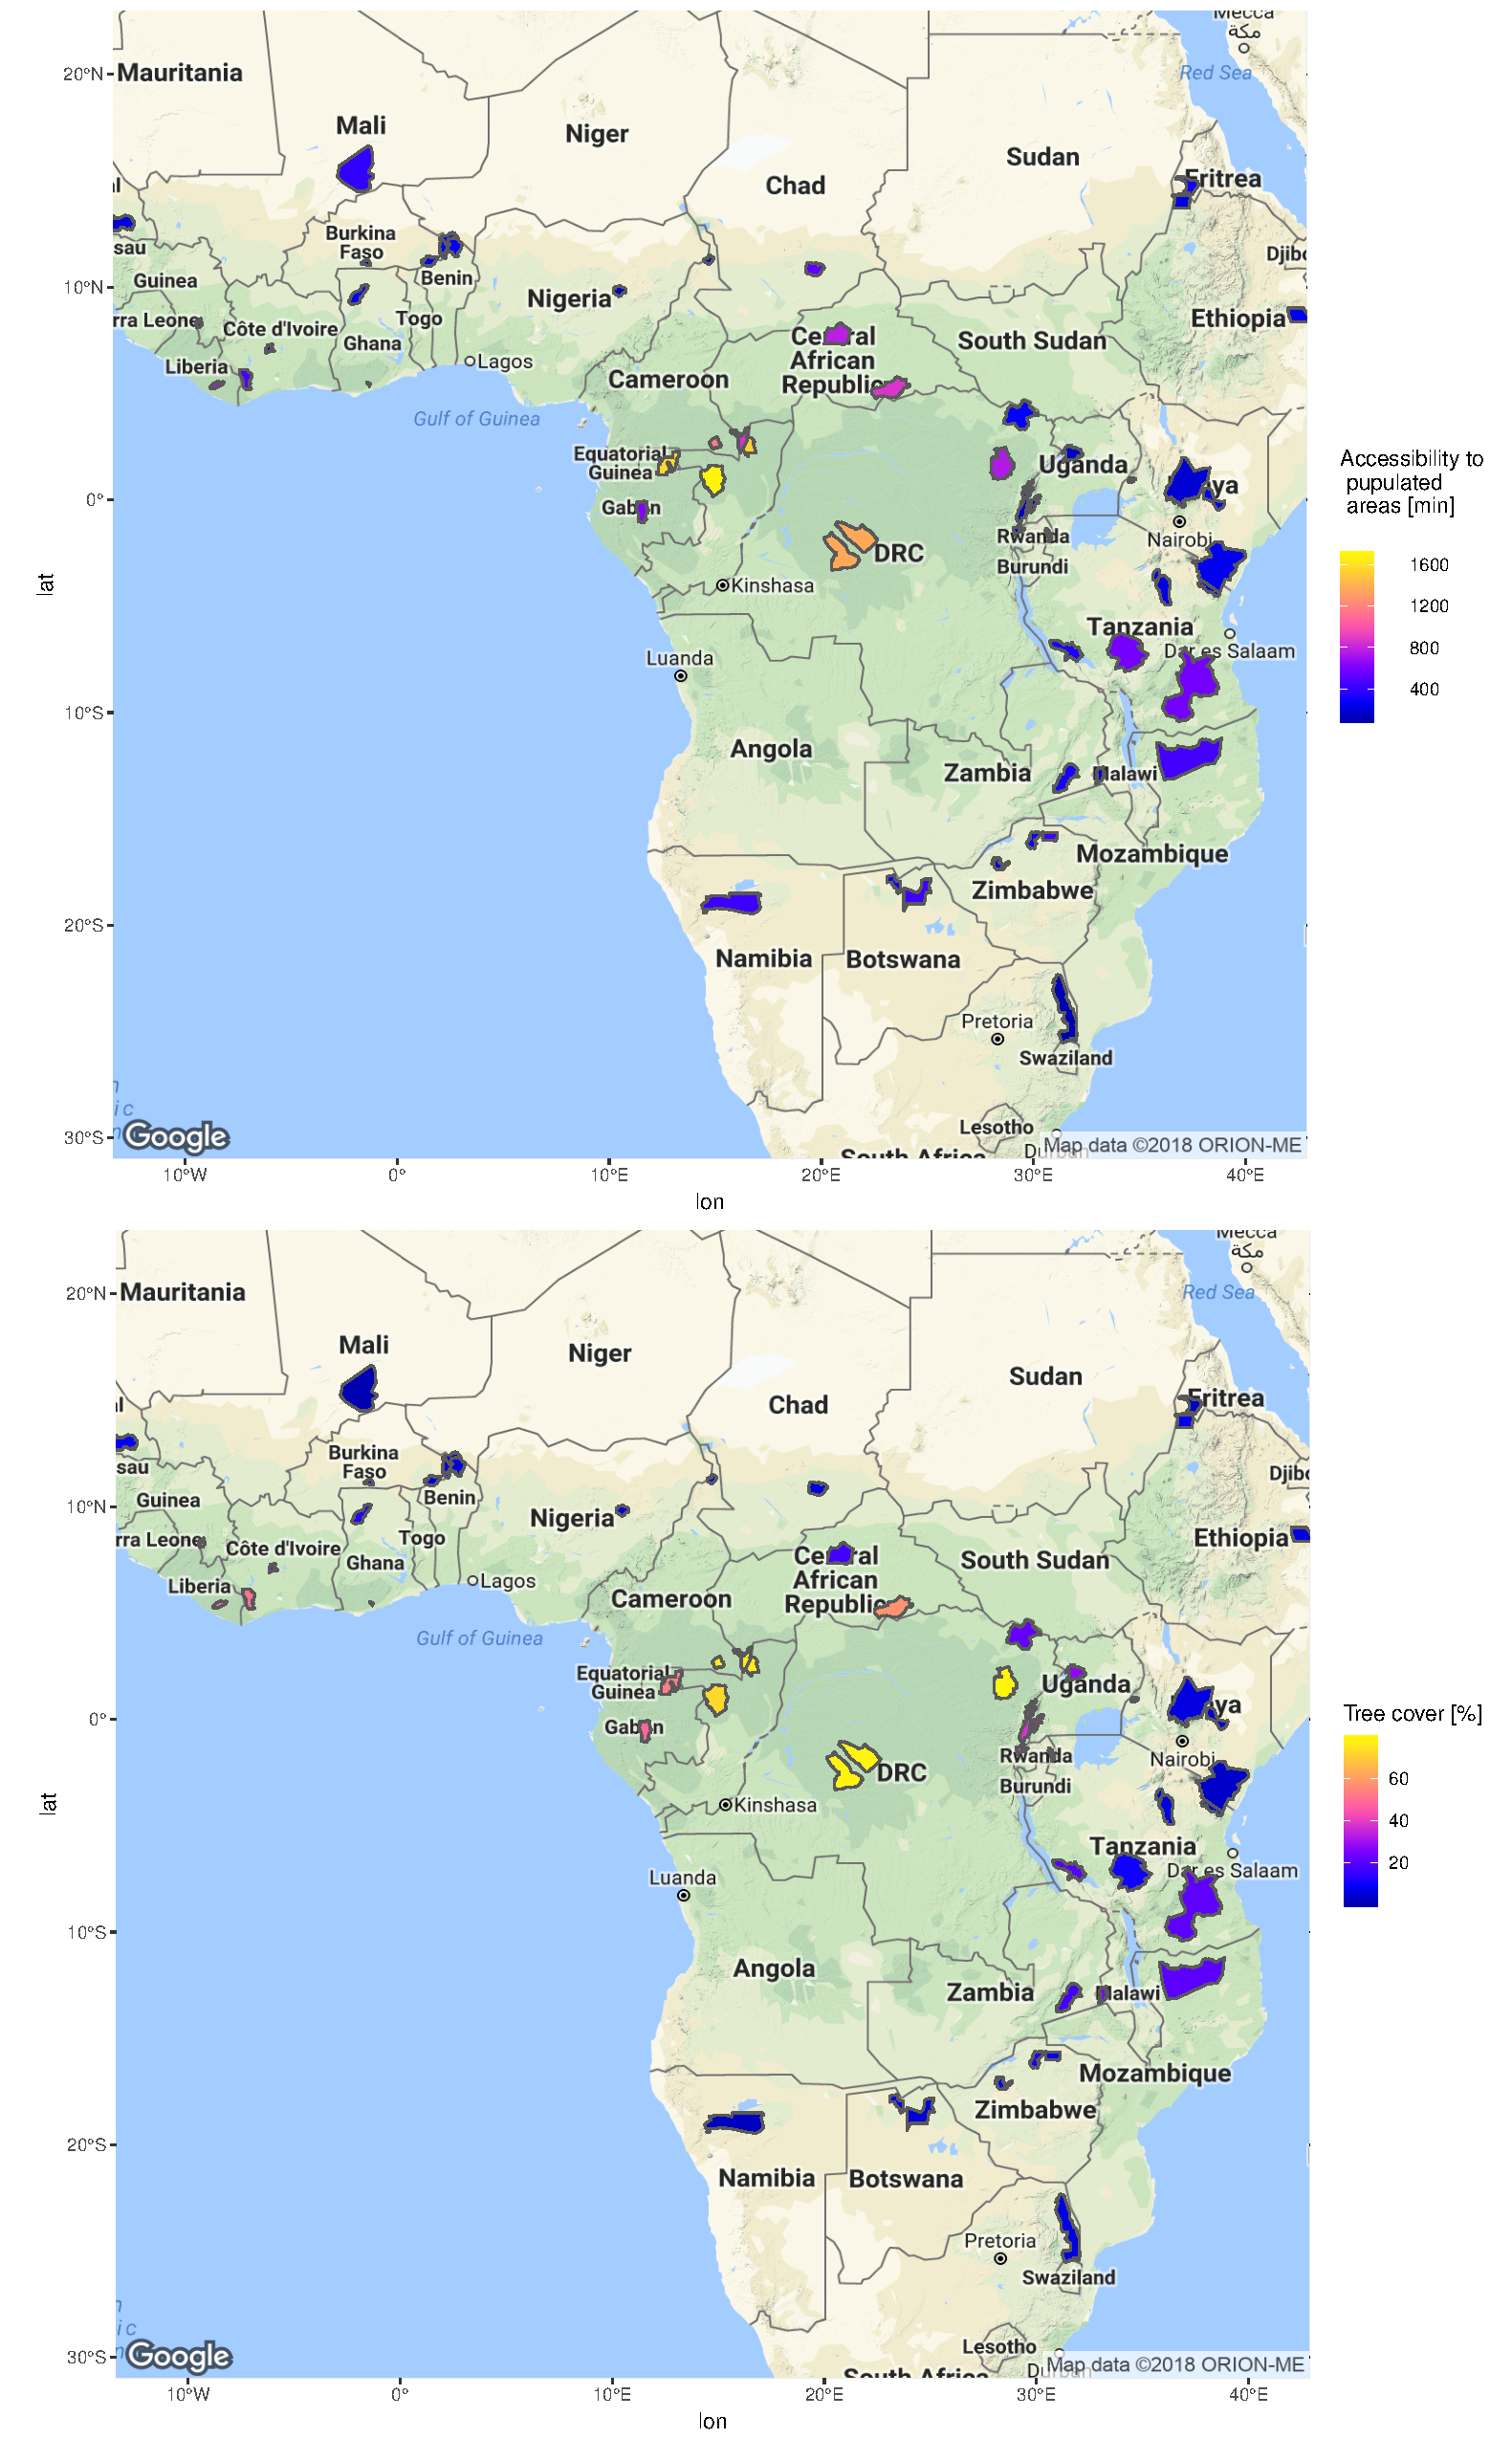
\includegraphics[width=14cm]{images/sample_session_1-cropped.pdf}
			\caption{On top the accessibility to the nearest populated areas in minutes and tree cover in percent at the bottom}
			\label{sample_session_1}
		\end{center}
	\end{figure}
	% \vskip 2em%
\end{center}


Figure \ref{sample_session_1} shows the mean tree cover in percent from 2000 to 2005 for each elephant territory in the upper figure and the mean accessibility of the territories in the figure at the bottom. Eye-catching but not surprising is the negative relationship between accessibility and tree cover resulting in a regional pattern with the highest tree cover and lowest accessibility found in central Africa, while toward the north, south and west, the accessibility increases and the tree cover decreases.

While this sample session shows the capabilities of the earthEngineGrabR package to aggregate over large areas, the next example is dedicated to the opposite situation. 

\section{Small-scale analysis}

\begin{wrapfigure}{r}{0.5\textwidth}
	\begin{center}
		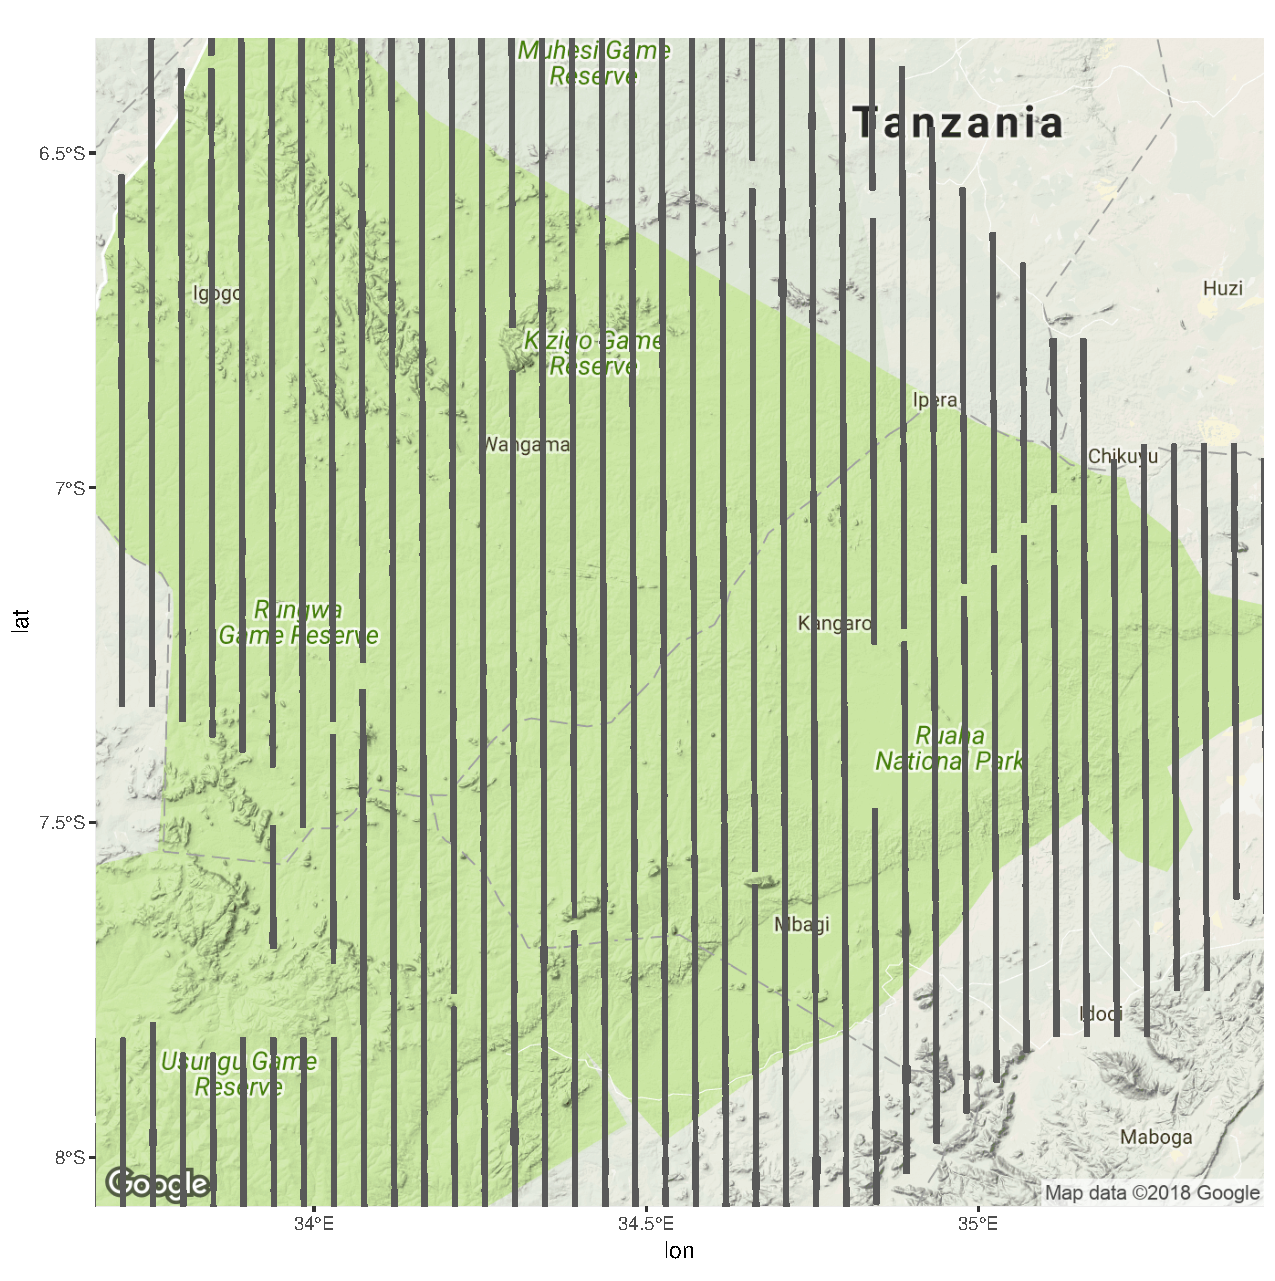
\includegraphics[width=7cm]{images/stripes-cropped.pdf}
		\caption{Spatial coverage of the aerial survey for Tanzania}
		\label{stripes}
	\end{center}
\end{wrapfigure}
% \vskip 2em%


Because of your access to the Great Elephant Census data you have not only the aggregated data for each territory but also the pre-aggregated survey data consisting of the number of elephants counted within a region specified by position, hight and the flight path of the aircraft. 


The combined areas form the spatial coverage of the survey and are available as shapefiles.
Figure \ref{stripes} shows the coverage for Tanzania. You are interested in the availability of surface water in each of these regions. Therefore you want to use the jrc-distance-to-surface-water data product available in the earthEngineGrabR package. 
As the target, you use the shapefile of the survey coverage and only specify the \texttt{jrc\_distanceToWater} product in the products argument. As spatial and temporal reducer you choose median. 

\begin{lstlisting}

africa_elephant_data_stripes <- ee_grab(
target = system.file("data/aerial-stripes.shp", package="earthEngineGrabR"), 
products = list(
eeProduct_jrc_distanceToWater(yearIntervall = c(2000,2000), spatialReducer = "median")
),
resolution = 50
)
\end{lstlisting}



Due to the smaller area of the features of the target (mean area of 0.7 km$^2$), you choose a resolution of 50 m and execute the function. The computation time takes about 3 m, and the result is shown in figure \ref{session_2}. Since the area of the coverage is too small for a meaningful visualisation, figure \ref{session_2} shows an actively zoomed view of the actual figure \ref{stripes}. 

\begin{center}
	\begin{figure}[h]
		\begin{center}
			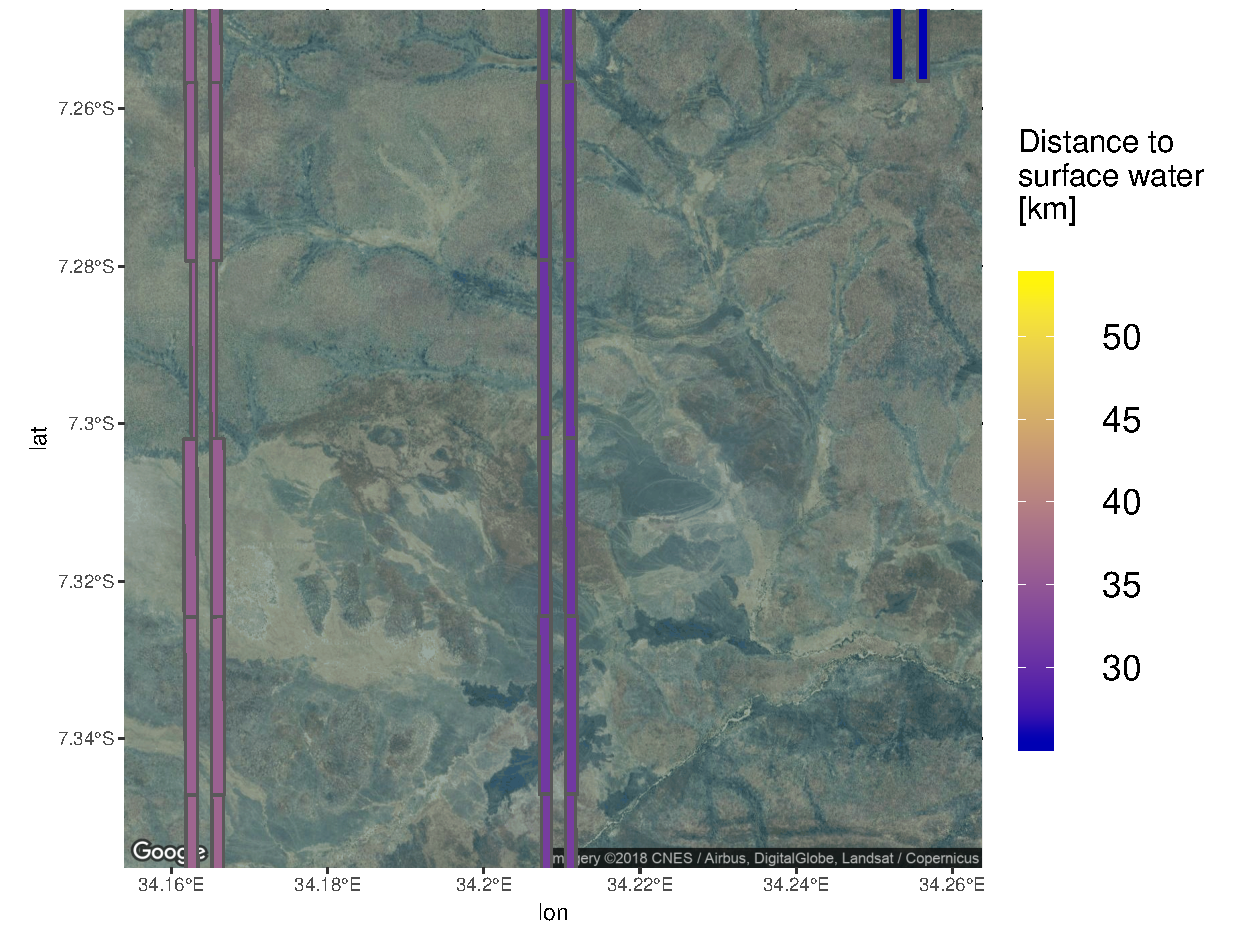
\includegraphics[width=15cm]{images/stripes_distance_2.pdf}
			\caption{Distance to surface water in km for the coverage of the areal survey}
			\label{session_2}
		\end{center}
	\end{figure}
	% \vskip 2em%
\end{center}

The distance to surface water is specified in km (though, the actual resolution is 50 m) and refers to the distance to the next Landsat pixel (30 m x 30 m) classified as water (\cite{pekel2016high}). The distance ranges from approximately 25 km to 35 km. In figure \ref{session_2} the aerial stripes on the left indicate a higher distance than the stripes on the right side of the map. Thus, the next close surface water must be located approximately 25 km in an eastward direction. 

This session shows the flexibility of the earthEngineGrabR referred to the scale of analysis and the shape of the AOI.

In the last example, a more extended use case of the \texttt{ee\_grab()} function is presented.

\section{Time-series analysis}

You are also interested in changes over time, for example, the change of precipitation in the elephant territories. Out of the documentation you know, that the precipitation product of the earthEngineGrabR is available from 2000 to 2015 on a yearly basis, thus you decide to calculate the precipitation for each year from 2000 to 2015 and analyse the change by using a linear model. The chirps-precipitation product is produced from satellite data on a daily basis, what offers the possibility to calculate the yearly precipitation sum. Because the yearly precipitation sum is a common practice in hydrology and compared to the mean not this prone to extreme values you decide to calculate the annual sum in each of the elephant territories for each year. To achieve that, you create one product for each year and pass the list of products to the \texttt{ee\_grab()} function.
The list of products can be generated using a vector of years from 2000 to 2015 and iterate the precipitation data product function over the years vector.

\begin{lstlisting}

years <- 2000:2015
products_ts <- list()

for (i in seq_along(years)) {
products_ts[[i]] <- eeProduct_chirps_precipitation(yearIntervall = c(years[i], years[i]), temporalReducer = "sum")
}

precipitation_time_series <- ee_grab(
target = system.file("data/territories.shp", package="earthEngineGrabR"),
products = products_ts,
resolution = 1000
)
\end{lstlisting}


As temporal reducer, you choose sum, and for the year interval, you take the i-th value of the created years vector. This generates a list of 15 specified data products for each year from 2000 to 2015. This list is passed to the products argument in the \texttt{ee\_grab()} function.
Due to the large-scale of your analysis, you again select a resolution of 1000 m. Since you want the spatial mean of the yearly precipitation sum in the territories, which already is the default spatial reducer, all necessary parameters in the \texttt{ee\_grab()} function are specified. While the processing of a single request for one year would take about 3 m, the processing time of all 15 data products require only approximately 15 m. Because the requests are sent and processed in parallel, the relationship of processing time and the number of requests is nonlinear. This point will be explained further in the discussion.

The output is an object of class sf that contains all properties of the original territories shapefile with 15 added columns for the precipitation sum of each year.
Next, you use a linear model of $year  \sim precipitation$ for each territory and retrieve the estimates for the effect of year. 

The estimates show the linear effect of year on the yearly precipitation sum in mm for each of the elephant territories. 
By joining the estimates with the spatial data of the territories, the estimates can be visualised spatially. 

\begin{center}
	\begin{figure}[h]
		\begin{center}
			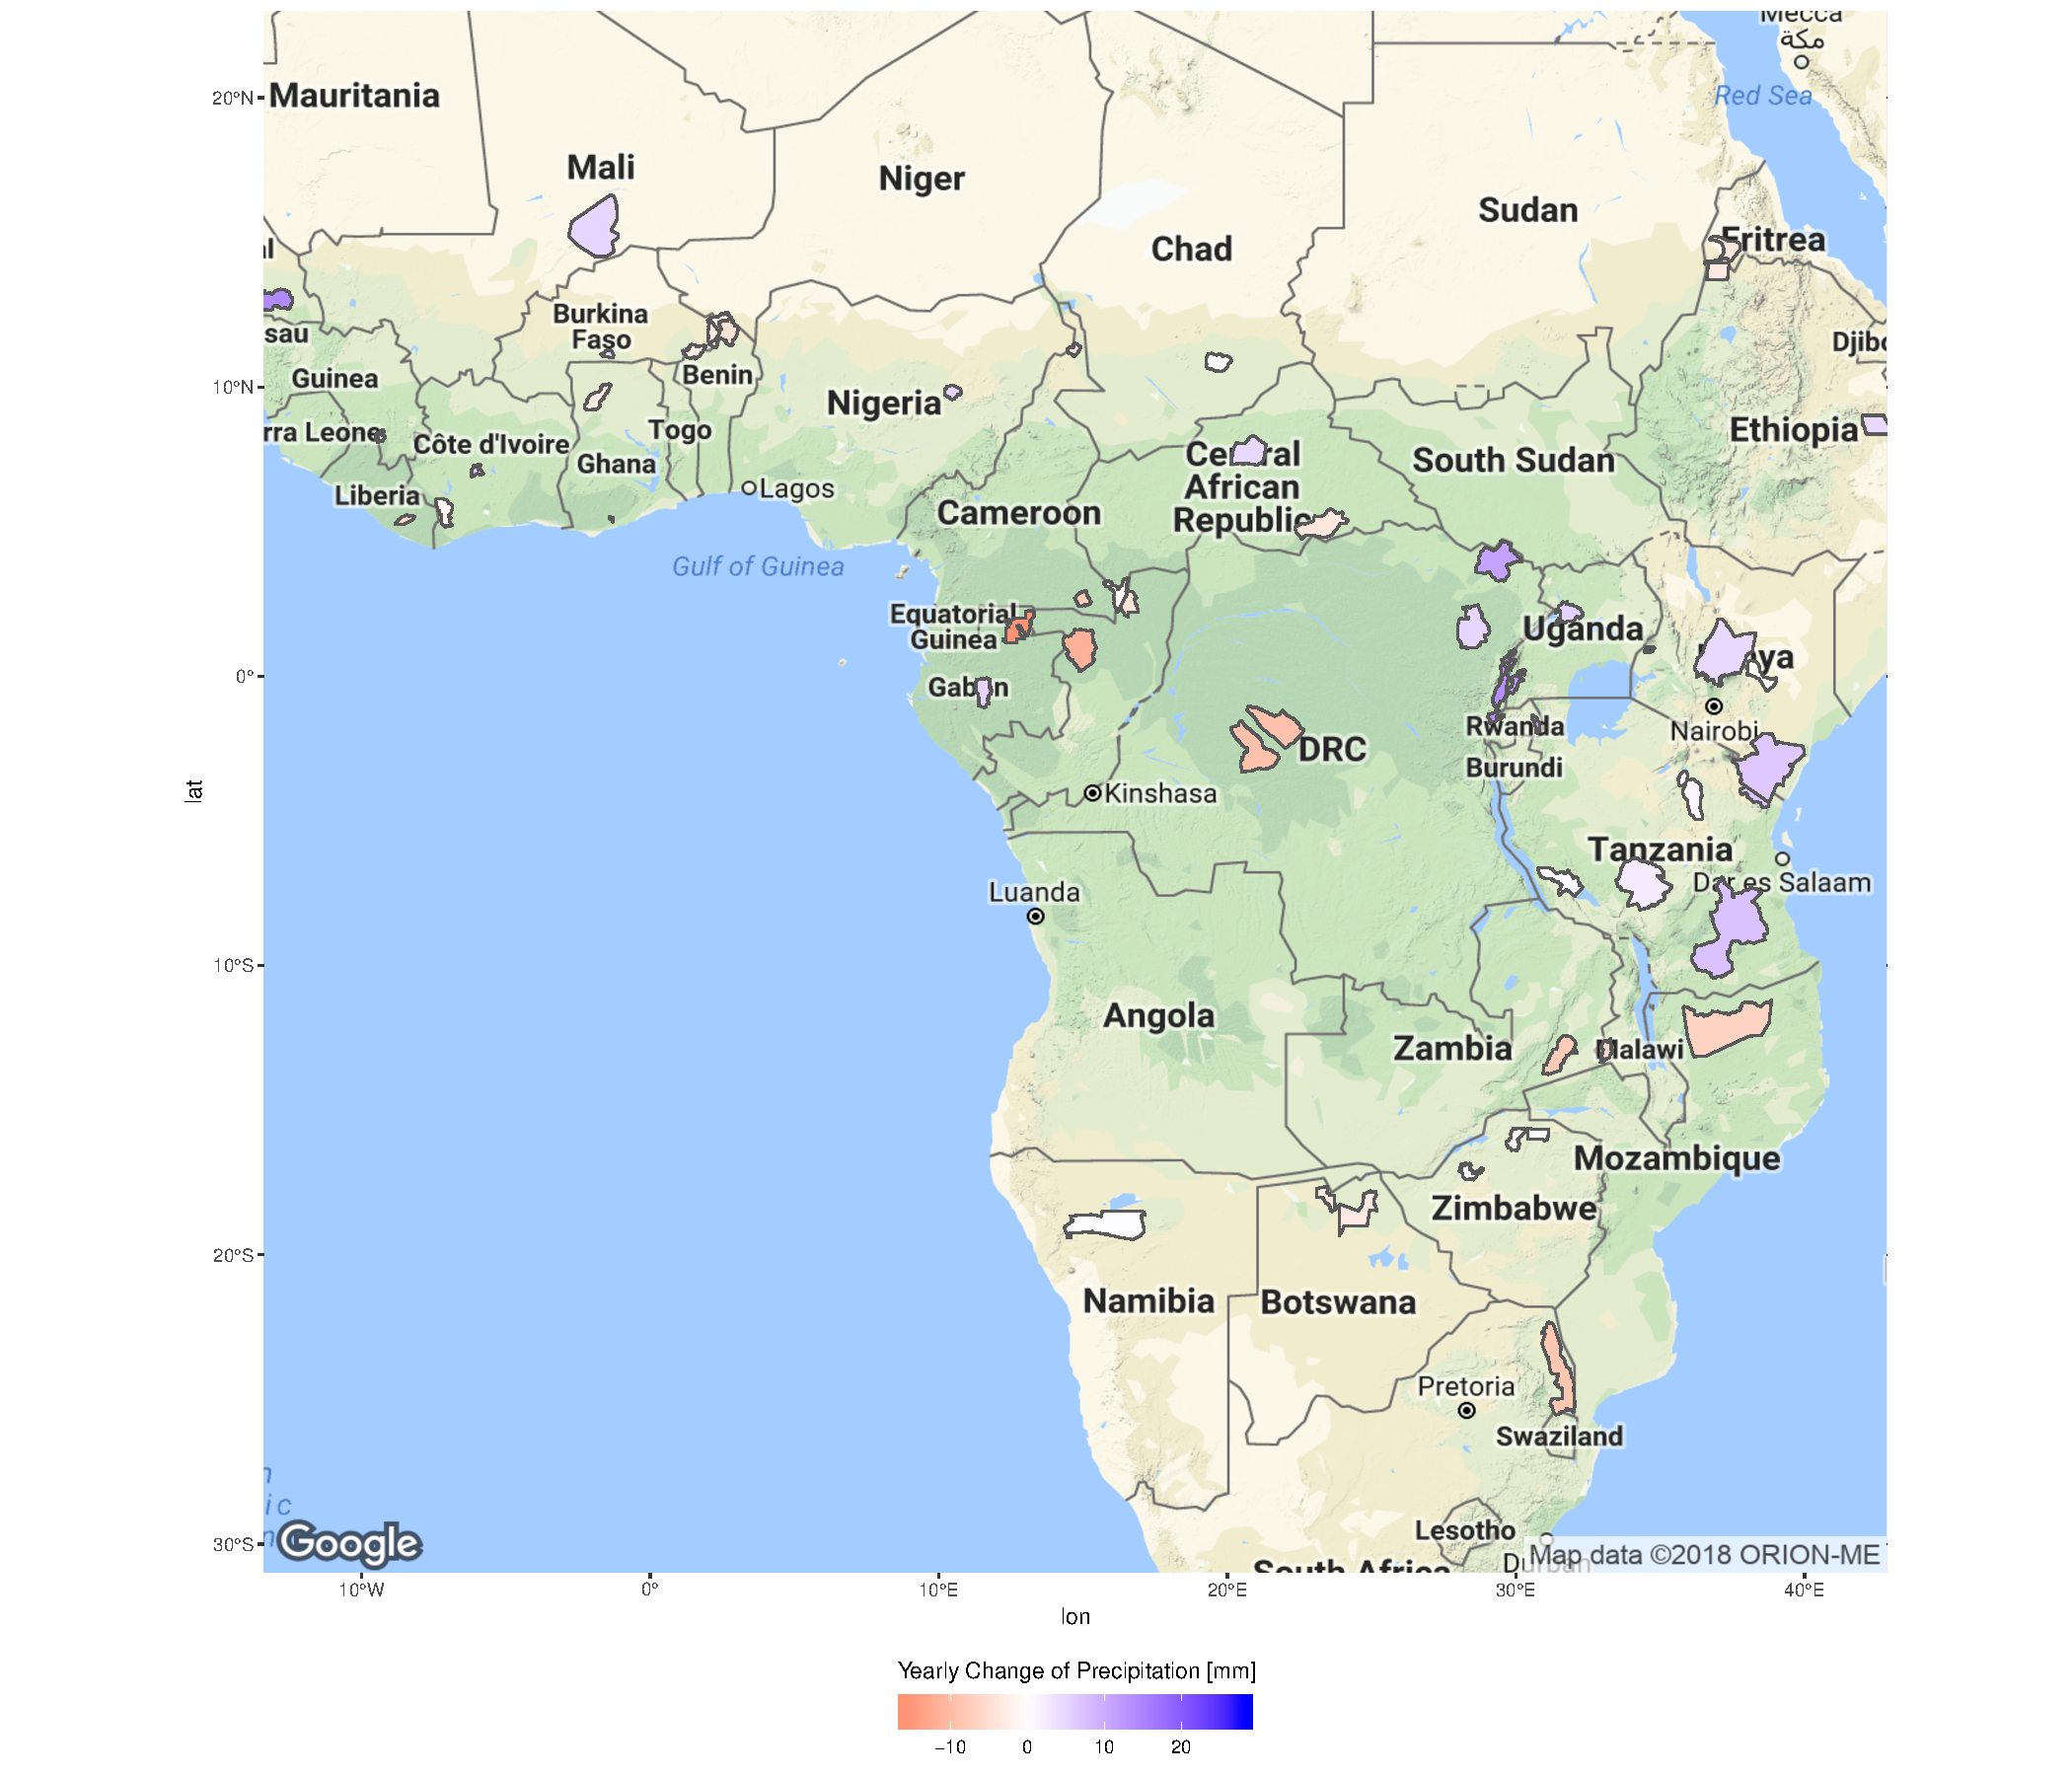
\includegraphics[width=16cm]{images/change_precipitation.pdf}
			\label{change}
		\end{center}
	\end{figure}
	% \vskip 2em%
\end{center}


Figure \ref{change} shows the estimate of the yearly change of the annual precipitation sum in mm for each territory. That estimates reflect a yearly change from - 10 mm to + 20 mm. While the yearly precipitation sum is increasing for the territories in East Africa, it is decreasing for most territories in central Africa, especially for those with hight tree cover (see figure \ref*{sample_session_1}).


\section{Summary}

The focus of this section is not on the interpretation of the results but to present the use of the earthEngineGrabR package.
With the use of the package, it was possible to quickly and easily acquire remote sensing data in three different use-cases. First, with the instructions on the packages Git Hup site, the requirements and the earthEngineGrabR were installed. Next, the \texttt{ee\_grab\_init()} installed the necessary Python dependencies and guided the user through the different authentications. The section illustrated how to use R, autocomplete feature and the package's data product functions to browse through the available data products and quickly open further documentation. Next, the \texttt{ee\_grab()} function was used to acquire remote sensing data according to 3 different questions and use-cases. The section showed the package's flexibility referring to the possible AOI, by obtaining data for both large-scale analyses with a mean area of the territories of 9862 km$^2$ and small-scale study with a mean area of 0.7 km$^2$.
The last sample session gave suggestions on how to extend the possibilities of the package by integrating the \texttt{ee\_grab()} over a series of years and doing this, acquire a time series of a specific data products.






